\section{Data Transmission Packet Processing Module}

To transmit data packets from the event bus, the network stack must
acquire the variable length packets, place them into larger udp
datagrams, set the metadata fields, and transmit them. However, we
must also save a copy of each packet (for possible retransmission),
and respond to a retransmission request should one occur during the
normal stream of data transmission.

To enable retransmission we have a packet TX FIFO with space for 256
1024-byte packets; a data packet should never exceed 600 bytes. This
FIFO also gives us headroom should the TX Fifo fill due to
insufficient access to the TX Mux interface. Note that, on average, we
have more than enough TX bandwidth -- but in the short run it is
possible to fill the TX fifo and thus need to buffer packets in the
in-memory FIFO.

This interface is heavily pipelined, as data bus packet transmission
is not viewed as an event-critical process.

We have various FIFOs and synchronization interfaces to guarantee our
goal of, within an ECYCLE, being able to service:

\begin{itemize}
\item The arrival of two new data bus packets and their subsequent
  memory writes to the fifo.
\item The placement of two packets in the memory fifo into the output
  FIFO for transmission
\item The retrieval of one packet for retransmission
\end{itemize}

 \begin{figure}
\begin{centering}
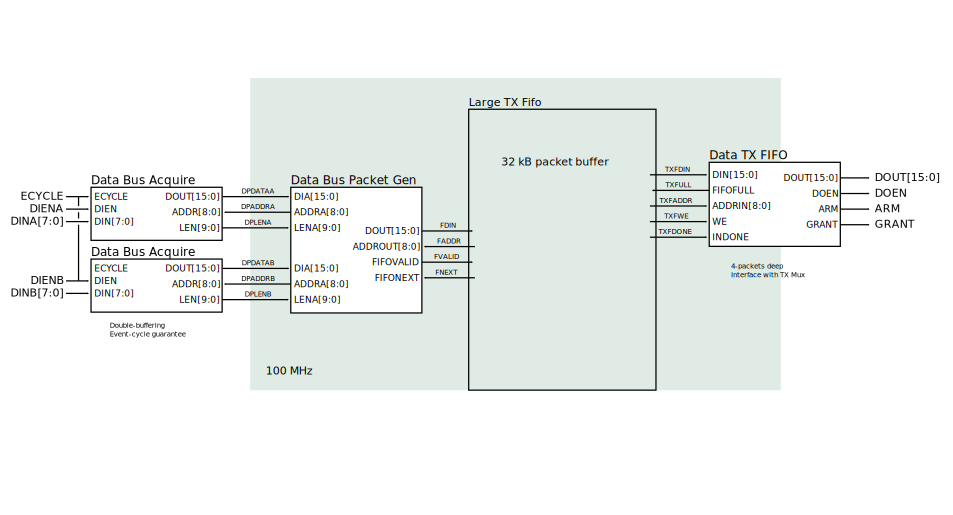
\includegraphics[scale=0.7]{data.svg}
\end{centering}
\caption{Data Transmission Interface}
\label{data}
\end{figure}


\subsection{Data Bus Acquire}
The data bus acquire interface takes a data bus packet and: 

1. event-cycle aligns it, so it is guaranteed to be available on the
   next ecycle.
2. converts it to a 16-bit-wide packet
3. measures the length

\subsubsection{Interface and Implementation} 
 \begin{figure}
\begin{centering}
\includegraphics[scale=0.8]{data.acquire.svg}
\end{centering}
\caption{Data Bus Acquire.}
\label{data.acquire}
\end{figure}

It uses a double-buffer approach. On the cycle following
\signal{ECYCLE}-assertion, \signal{LEN[9:0]} contains the length of
the packet in words, not bytes; if \signal{LEN[9:0]} =0 then there is
no packet awaiting transmission.

\signal{BSEL} selects which buffer. \signal{ADDR[8:0]} selects the
output word.

\subsection{Data Bus Packet Gen}
The data bus packet generator generates one or two datagrams every
event cycle, which are ready for processing at the end of the event
cycle.
The data bus packet generator also assigns the 32-bit sequence ID to
each packet based upon packet source and type.


\subsubsection{Interface}
\begin{figure}
\begin{centering}
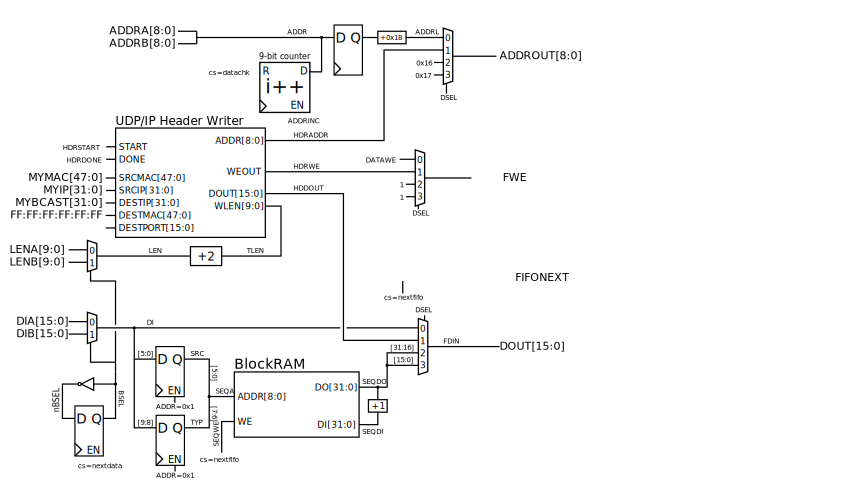
\includegraphics[scale=0.8]{data.packetgen.svg}
\end{centering}
\caption{Data Bus Transmission packet generation.}
\label{data.packetgen}
\end{figure}

\begin{figure}
\begin{centering}
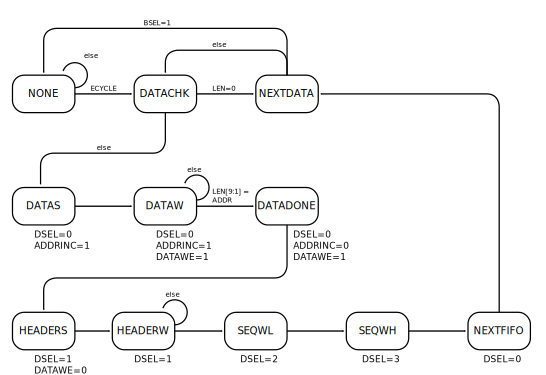
\includegraphics[scale=0.8]{data.packetgen.fsm.svg}
\end{centering}
\caption{Data Bus Transmission packet generation finite state machine.}
\label{data.packetgen.fsm}
\end{figure}

The input interface interoperates with the Data Bus Acquire module.
Output packets are simply written to the downstaream FIFO. 



\subsubsection{implementation}
To store a packet, we examine both \signal{LENA[9:0]} and
\signal{LENB[9:0]} to check for non-zero values each Event Cycle.
Should a packet have a non-zero value, we begin copying it into the
output FIFO. Througout the transmission of this packet, we lock on to
the packet source and type, and use this to look up the current value
of sequence number via \signal{SEQDO[31:0]} .

Then, we use the UDPheader to write the relevant packet header data.
\signal{TLEN } is two greater than the input \signal{LEN[9:0]} to
account for the addition of the sequence ID in the header. The
destination port is calculated from the latched \signal{SRC[5:0]} and
\signal{TYP[1:0]}.

Finally, the sequence ID is written to the fifo and the packet is
committed by incrementingthe input fifo pointer, \signal{FADDR[10:9]}.

The fifo output stage, running at 100 MHz, simply checks if the input
fifo pointer (registered as \signal{FIFONUM}) is different from the
output fifo pointer and asserts \signal{FIFOVALID} if so.

\subsection{Memory Arbitration}
\begin{figure}
\begin{centering}
\includegraphics[scale=0.8]{data.memarbit.svg}
\end{centering}
\caption{Data Bus Transmission memory arbitration interface}
\label{data.memarbit}
\end{figure}

\begin{figure}
\begin{centering}
\includegraphics[scale=0.8]{data.memarbit.fsm.svg}
\end{centering}
\caption{Data Bus Transmission memory arbitration interface finate state machine.}
\label{data.memarbit.fsm}
\end{figure}

The data memory arbitration module controls access to the NoBL-based
RAM used as a pacet FIFO. Each component has exclusive access to the
memory pending the arbitrator's assertion of the associated
\signal{START} signal. This access is yielded when the \signal{DONE}
signal for the submodule goes high. All submodules run at 100 MHz, and
are expected to internally compensate for read and write latencies to
the RAM.

All modules involved read the value of the \signal{BP[7:0]} (Base
Pointer) signal, which indicates the next FIFO location to be written.
For example, BP = 0x32 if FIFO location 0x31 was just written to.

There are three primary modules: 
\begin{enumerate}
\item \textbf{Memory Packet Input} : writes the packet into memory,
  extracting out the SRC, TYP, SEQ, and passing those onto the
  retransmission lookup module for storage.
\item \textbf{Retransmission Lookup} : This module interfaces to the
  external retransmission packet processing module, taking in
  retransmission requests and looking up the expected packet in the
  RAM FIFO.
\item \textbf{Memroy Packet Transmission} : When the RAM FIFO is
  non-empty this module reads out packets and writes them to the Data
  Output FIFO.
\end{enumerate}

\subsubsection{Memory Packet Input}
\begin{figure}
\begin{centering}
\includegraphics[scale=0.8]{memarbit.pktinput.svg}
\end{centering}
\caption{Data Bus Transmission memory arbitration interface packet input module.}
\label{memarbit.pktinput}
\end{figure}

\begin{figure}
\begin{centering}
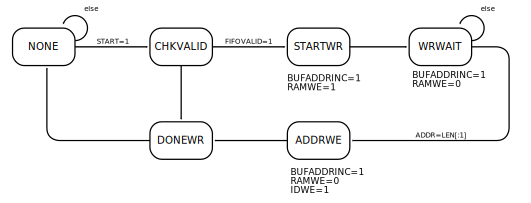
\includegraphics[scale=0.8]{memarbit.pktinput.fsm.svg}
\end{centering}
\caption{Data Bus Transmission memory arbitration interface packet input module finate state machine} 
\label{memarbit.pktinput.fsm}
\end{figure}

Assertion of \signal{START} instructs the memory packet input to
determine if the contents of the upstream FIFO are valid
(\signal{FIFOVALID} is asserted). If so, the packet is read out, with
one-cycle latency between \signal{ADDROUT[8:0]} and
\signal{DIN[15:0]}.

 The relevant packet metadata is extracted based on
address, and the packet is written to the FIFO beginning at the
location of the current base pointer (\signal{BP[7:0]}). Completion of
this results in the assertion of \signal{DONE} and the incrementing of
\signal{BP} to indicate the new FIFO contents.  Additionally, the
packet metadata and fifo location are written to the Retransmission
Lookup module via the assertion of \signal{IDWE}.

\subsubsection{Memory Packet Retransmission Lookup} 
\begin{figure}
\begin{centering}
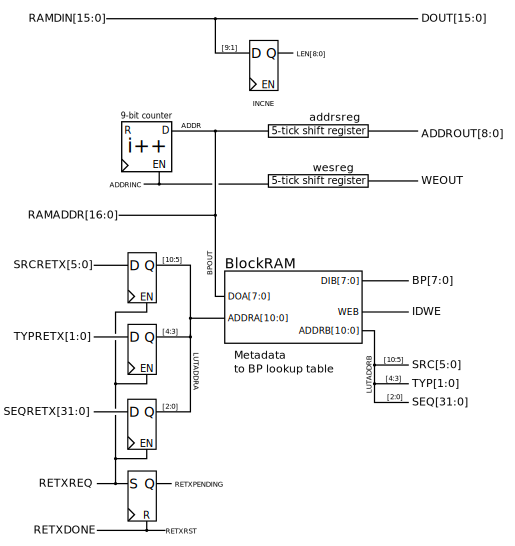
\includegraphics[scale=0.8]{memarbit.retx.svg}
\end{centering}
\caption{Data Bus Transmission memory arbitration interface retransmission lookup.}
\label{memarbit.retx}
\end{figure}

\begin{figure}
\begin{centering}
\includegraphics[scale=0.8]{memarbit.retx.fsm.svg}
\end{centering}
\caption{Data Bus Transmission memory arbitration interface retransmission lookup finite state machine.}
\label{memarbit.retx.fsm}
\end{figure}

When servicing a retransmission request, this module has an internal
lookup where it stores the BP locations for the eight most recent
packets of a given (source, type). Of course, the FIFO can't actually
hold all of those packets, and some sources may produce more packets
per unit time than others, resulting in a FIFO with far more packets
from (7, 2) than (3, 0). So the FIFO location that the lookup table
points to might no longer contain the relevant packet.

The Memory  Packet Retransmission Lookup  module does not  worry about
this case,  and simply  passes the  data downstream. It  is up  to the
retransmission  packet  processing module  to  check  that the  packet
pulled  out of  the FIFO  is the  one it  is looking  for,  and return
success or failure accordingly.
 

This module serves two masters: The ReTX Packet Processing Module and
the main controller. Should the ReTX packet Processing module request
a packet for retransmission by asserting \signal{RETXREQ} (which
additionally latches the relevent RTX packet metadata), the module
must wait until the assertion of \signal{START} to act on it.

While \signal{IDWE} may be asserted at any time, the round-robin
nature of the memory arbitration system eliminates the possibility of
race conditions.

DATA is read out of RAM using the combined looked-up BP and the
internal \signal{ADDR[8:0]}. Due to the latency created by both the
registering of RAM IO and the NoBL Pipelined RAM itself, shift
registers are used to assert that the values written to the ReTx
Packet Processing Module are correctly aligned.

\subsubsection{Memory Packet Transmission}
\begin{figure}
\begin{centering}
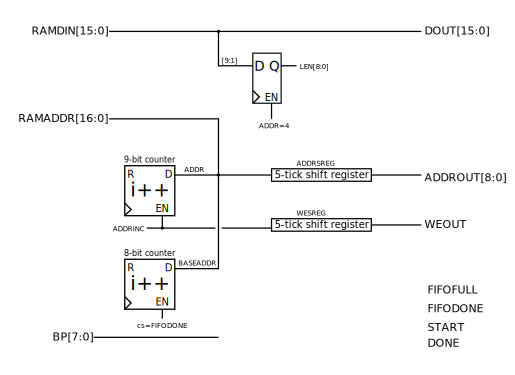
\includegraphics[scale=0.8]{memarbit.pktoutput.svg}
\end{centering}
\caption{Data Bus Transmission memory arbitration interface retransmission lookup.}
\label{memarbit.retx}
\end{figure}

\begin{figure}
\begin{centering}
\includegraphics[scale=0.8]{memarbit.pktoutput.fsm.svg}
\end{centering}
\caption{Data Bus Transmission memory arbitration interface retransmission lookup finite state machine.}
\label{memarbit.retx.fsm}
\end{figure}

Structurally this module is very similar to the Retransmission Lookup
module, except that it contains an internal BP (called
\signal{BASEADDR[7:0]}) which is compared to the input
\signal{BP[7:0]} to determine if the RAM FIFO contains data.  If this
is the case and if the output fifo is not full (\signal{FIFOFULL} is
not asserted) then the packet is read from the RAM FIFO and written
into the output FIFO. \signal{FIFODONE} is asserted upon completion of
this write process.


\subsection{Data Output FIFO}
The data output fifo is the fifo that buffers data packets to be
transmitted to deal with the fact that while our Data TX hit rate is
only 64 packets out of every 100 slots (1 ms) we could have them all
bunch up, and that would be, in the words of T-Rex ``most
unfortunate''.

The fifo is constrained to -always- take input from the packet
generator, and presents a series of 1k-deep packet interfaces.




\begin{figure}
\begin{centering}
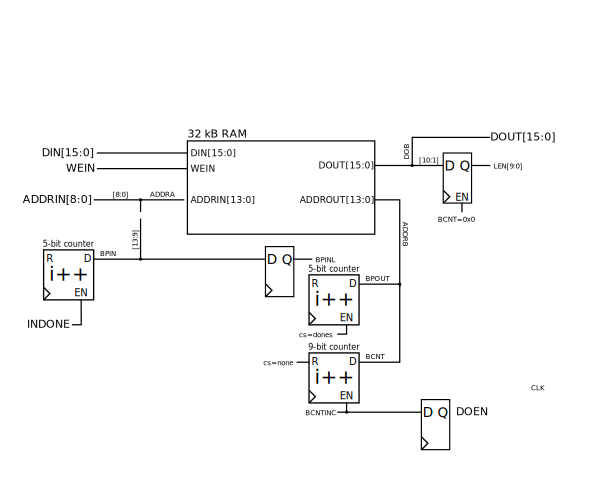
\includegraphics[scale=0.8]{data.outputfifo.svg}
\end{centering}
\caption{Data Bus Transmission output FIFO.}
\label{data.outputfifo}
\end{figure}
